\chapter{Zielbestimmung}

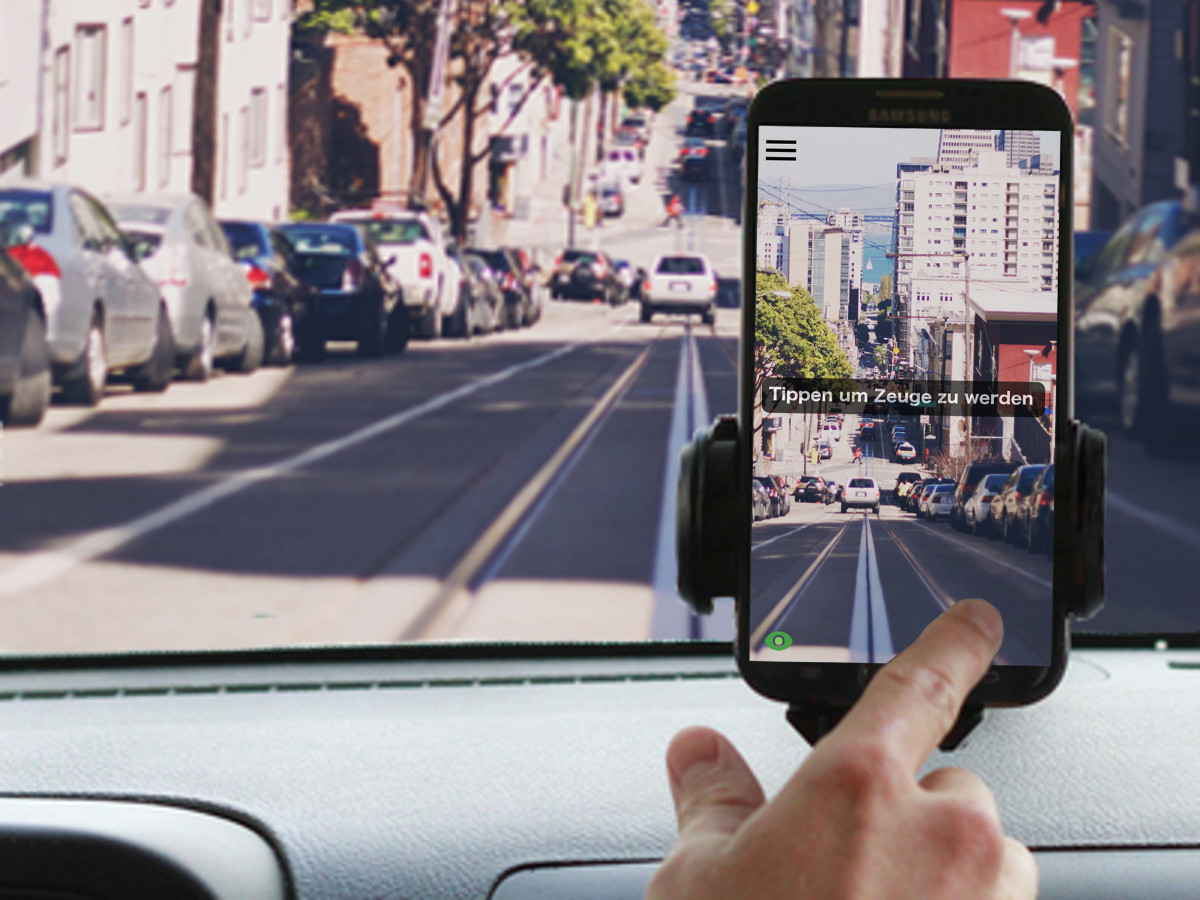
\includegraphics[width=\textwidth]{subtopicsFuncspec/Res//Mockups/Portrait_camera_view_car.jpg}\\[0.5cm]

Das Produkt ermöglicht es seinen Nutzern ihre Autofahrten zu überwachen, indem es durch die \gls{Smartphone}kamera den Straßenverkehr verfolgt und relevantes Videomaterial \glslink{persistieren}{persistent} abspeichert. Dieses wird bei Bedarf verwendet, um Unfallhergänge im Straßenverkehr zu dokumentieren. Dabei gilt es, dem deutschen Datenschutzrecht gerecht zu werden, indem Personen und personenbezogene Daten, wie zum Beispiel Autokennzeichen, unkenntlich gemacht werden. Die Anwendung bietet dem Nutzer dafür eine moderne und intuitive Bedienoberfläche.\newline
Zur Realisierung kann das Produkt in drei Hauptbestandteile aufgegliedert werden: Die \gls{Android} \gls{App}, den \gls{Web-Dienst} und das \gls{Web-Interface}. Diese Aufteilung wird in diesem Heft um Übersicht zu schaffen auch in nachfolgenden Kapiteln beibehalten.

\section{Musskriterien}
\subsection{App}
	\begin{enumerate}
	\renewcommand{\labelenumi}{\textbf{\theenumi}}
	\renewcommand{\theenumi}{PK\arabic{enumi}0}
	\setcounter{enumi}{99}
	\item Nutzer müssen sich anmelden um die \gls{App} zu verwenden
	\item Nur registrierte Nutzer können die \gls{App} verwenden
	\item Der Straßenverkehr wird durch die \gls{Smartphone}kamera beobachtet 
	\item Relevante Videodaten werden verschlüsselt abgespeichert
	\item Relevante Daten werden durch Auswertung der Sensordaten des \glspl{Smartphone} erkannt. Hierbei werden die Werte des G-Sensors ausgewertet
	\item Während der Aufnahme werden sämtliche Nutzereingaben und \gls{G-Sensor}daten ignoriert
	\item Videodaten speichern relevante \gls{Metadaten}
	\item Es wird ab dem \gls{App}start mit dem Beobachten des Straßenverkehrs begonnen
	\item Es wird nur das Hochformat unterstützt
	\item Die Beobachtung läuft nur während sich die \gls{App} im Vordergrund befindet
	\item Videodaten werden verschlüsselt, sobald sie \glslink{persistieren}{persistiert} werden
	\item Verschlüsselte Videodaten werden aufgelistet
	\item Verschlüsselte Videodaten können gelöscht werden
	\item Vom Nutzer ausgewählte verschlüsselte Videodaten werden an einen \gls{Web-Dienst} gesendet, der diese \glslink{anonymisieren}{anonymisiert}
	\item Geräte, auf denen \gls{Android} \gls{API} Level 19 (Android 4.4) und höhre läuft werden unterstützt
	\item Die Benutzeroberfläche wird für Geräte ab einer Displaydiagonale von 4 Zoll optimiert
	\item Wenn verschlüsselte Videodateien lange Zeit nicht zum \gls{anonymisieren} ausgewählt wurden, wird der Nutzer benachrichtigt, dass er diese löschen kann
	\item Die aufnahmespezifischen Einstellungen werden angezeigt
	\item Die Standardsprache ist Deutsch
	\end{enumerate}
\subsection{Web-Dienst}
	\begin{enumerate}
	\renewcommand{\labelenumi}{\textbf{\theenumi}}
	\renewcommand{\theenumi}{PK\arabic{enumi}0}
	\setcounter{enumi}{199}
	\item Es existiert eine Schnittstelle, um Videodaten hochzuladen
	\item Von der \gls{App} gesendete Videodaten werden \glslink{anonymisieren}{anonymisiert}
	\item Nach Abschluss der \glslink{anonymisieren}{Anonymisierung} wird der Nutzer per \gls{E-Mail} benachrichtigt
	%\item Nach einer Registrierung bekommt der Nutzer eine Verifizierungs-E-Mail zugesendet
	\item Es existiert eine Schnittstelle, um Nutzeraccounts anzulegen
	\item Es existiert eine Schnittstelle, um Nutzeraccounts zu verwalten
	\item Es existiert eine Schnittstelle, um die Videodaten eines Nutzers verwalten zu können
	\item Nutzer müssen ihre \gls{E-Mail}-Adresse verifizieren um sich anmelden zu können
	\item Die Kommunikation zwischen App und Web-Dienst wird durch eine REST-\gls{API} realisiert
	\item Die Kommunikation zwischen \gls{Web-Interface} und \gls{Web-Dienst} wird durch eine REST-\gls{API} realisiert
	\item Es existiert eine obere Schranke für die Anzahl der Videodateien, die ein Nutzer zur gleichen Zeit auf seinem Nutzeraccount online speichern kann
	\item Passwörter werden nur als \gls{Hash-Code} abgespeichert
	\item Es wird Jetty verwendet
	\end{enumerate}
\subsection{Web-Interface}
	\begin{enumerate}
	\renewcommand{\labelenumi}{\textbf{\theenumi}}
	\renewcommand{\theenumi}{PK\arabic{enumi}0}
	\setcounter{enumi}{299}
	\item Es können Nutzeraccounts angelegt werden
	\item Es können Nutzeraccounts verwaltet werden
	\item Es können Videodaten verwaltet werden
	\item Es können Videodaten heruntergeladen werden
	\item Nur eingeloggte Nutzer haben Zugriff auf ihre Nutzerdaten
	\item Es können Passwort und \gls{E-Mail}-Adresse geändert werden
	\item Die Standardsprache ist Deutsch
	\end{enumerate}

\section{Wunschkriterien}
\subsection{App}
	\begin{enumerate}
	\renewcommand{\labelenumi}{\textbf{\theenumi}}
	\renewcommand{\theenumi}{WK\arabic{enumi}0}
	\setcounter{enumi}{99}
	\item Falls es \gls{Android} zulässt wird die Beobachtung auch ausgeführt, wenn sich die \gls{App} im Hintergrund befindet
	\item Sowohl Quer- als auch Hochformat werden unterstützt
	\item Die Beobachtung kann manuell gestartet und gestoppt werden
	\item Die Aufnahme kann manuell gestartet werden, auch wenn der \gls{G-Sensor} des Smartphones keinen Anlass dazu gibt
	\item Während der Aufnahme wird eine Möglichkeit angeboten die Aufnahme abzubrechen
	\item Es können Nutzeraccounts angelegt werden
	\item Es können Nutzeraccounts verwaltet werden
	\item \glslink{anonymisieren}{Anonymisierte} Videodateien können vom Server gelöscht werden
	\item Push-Benachrichtignungen vom \gls{Web-Dienst} werden angezeigt
	\item Es können Hilfestellungen für die Bedienung der \gls{App} angezeigt werden
	\item \glslink{anonymisieren}{Anonymisierte} Videodateien können heruntergeladen werden
	\item \glslink{anonymisieren}{Anonymisierte} Videodateien die zum Download bereit stehen und sich nicht auf dem \gls{Smartphone} befinden werden aufgelistet
	\item \glslink{anonymisieren}{Anonymisierte} Videodateien die sich auf dem \gls{Smartphone} befinden  werden aufgelistet
	\item \glslink{anonymisieren}{Anonymisierte} Videodateien können vom Speicher des \glspl{Smartphone} gelöscht werden
	\item \glslink{anonymisieren}{Anonymisierte} Videodateien die sich auf dem \gls{Smartphone} befinden können angesehen werden
	\item Die aufnahmespezifischen Einstellungen können bearbeitet werden
	\item So lange der \gls{G-Sensor} des Smartphones anlass zur Aufnahme gibt wird weiter aufgenommen
	\end{enumerate}
\subsection{Web-Dienst}
	\begin{enumerate}
	\renewcommand{\labelenumi}{\textbf{\theenumi}}
	\renewcommand{\theenumi}{WK\arabic{enumi}0}
	\setcounter{enumi}{199}
	\item Die Zeit, die die \glslink{anonymisieren}{Anonymisierung} in Anspruch nehmen wird, wird geschätzt und an den Nutzer weitergeleitet
	\item Es wird eine Push-Benachrichtigung an das \gls{Smartphone} gesendet, sobald die Anonymisierung der Videodaten abgeschlossen ist
	\item Videodaten werden maximal vier Wochen gespeichert
	\item Der Nutzer erhält eine Woche bevor ein Video glöscht wird eine \gls{E-Mail}-Banchrichtigung
	\end{enumerate}
\subsection{Web-Interface}
	\begin{enumerate}
	\renewcommand{\labelenumi}{\textbf{\theenumi}}
	\renewcommand{\theenumi}{WK\arabic{enumi}0}
	\setcounter{enumi}{299}
	\item Das Produkt wird neuen Nutzern präsentiert
	\item Nutzer können ihre anonymiserten Videos online ansehen
	\end{enumerate}

\section{Abgrenzungskriterien}
	\begin{enumerate}
	\renewcommand{\labelenumi}{\textbf{\theenumi}}
	\renewcommand{\theenumi}{AK\arabic{enumi}0}
	\item Das betrachten nicht \glslink{anonymisieren}{anonymisierter} Videodaten ist nicht möglich
	\item Videodaten werden nicht automatisch persistiert sobald die Beobachtung läuft
	\item \glspl{Livestream} werden nicht unterstützt
	\item Die \glslink{anonymisieren}{Anonymisierung} findet nicht auf dem \gls{Smartphone} statt
	\item Der \gls{Web-Dienst} speichert Videodaten nicht auf unbegrenzte Zeit und in unbegrenzter Anzahl
	\item Vom Speicher des Smartphones werden Videodaten nicht automatisch gelöscht
	\item Von Nutzern zurückgelegte Wege und besuchte Orte werden nicht aufgezeichnet
	\item Die \gls{App} ist nicht mit Windows Phone und iOS kompatibel
	\item Die \gls{App} wird nicht für Tablets optimiert
	\end{enumerate}